\section{Exploración de Datos}
\label{sec:exploracion_datos}

Con el fin de comprender la estructura y el comportamiento de los tres conjuntos de datos seleccionados, se ejecutaron nueve elementos de análisis exploratorio de datos (EDA) sobre el clúster de Apache Spark (\texttt{spark://10.195.34.34:7077}), combinando agregaciones distribuidas en PySpark con visualizaciones estadísticas. A continuación se presentan los hallazgos.

\subsection{Elemento 1 --- Reporte de calidad de datos: valores faltantes}
\label{subsec:eda_elemento1}

Se realizó un conteo distribuido de valores nulos y cadenas vacías por columna en los tres conjuntos de datos. En \textit{NYPD Arrest Data} ($141,870$ filas) se identificaron valores faltantes marginales, concentrados en \texttt{LAW\_CAT\_CD} ($869$ registros entre vacíos y el literal \texttt{'(null)'}, equivalentes al $0.61\%$), \texttt{PD\_DESC}, \texttt{OFNS\_DESC} y \texttt{KY\_CD} ($24$ casos cada uno, $0.02\%$), y \texttt{PD\_CD} y \texttt{LAW\_CODE} ($5$ casos, $0.00\%$). En \textit{Motor Vehicle Collisions} ($2,305,623$ filas en el corte consolidado, frente a $2,269,188$ en el corte inicial) se observó un patrón de faltantes estructural en los campos de vehículos secundarios (\texttt{VEHICLE TYPE CODE 5} con $99.56\%$ de nulos, \texttt{CONTRIBUTING FACTOR VEHICLE 5} con $99.54\%$, y los campos de los vehículos 3 y 4 entre $92.74\%$ y $98.40\%$), explicable porque la gran mayoría de las colisiones involucran solo uno o dos vehículos. Asimismo, se detectaron faltantes relevantes en variables administrativas de ubicación (\texttt{ZIP CODE} con $30.41\%$ y \texttt{BOROUGH} con $29.27\%$, frente a solo $10.44\%$ de nulos en \texttt{LATITUDE}/\texttt{LONGITUDE}). En \textit{NYCgov Poverty Measure Data} ($68,273$ filas) destacan los faltantes por salto lógico de la encuesta en \texttt{ENG} ($55.01\%$), \texttt{JWTR} ($51.20\%$), \texttt{WKW} ($45.98\%$), \texttt{ESR} ($17.28\%$) y \texttt{MSP} ($16.14\%$).

\begin{figure}[H]
    \centering
    \begin{minipage}[c]{0.46\textwidth}
        \centering
        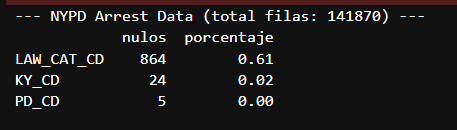
\includegraphics[width=\linewidth]{imagenes/image.png}\\[0.25cm]
        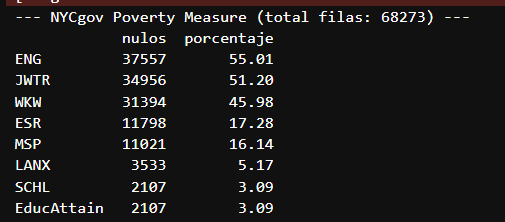
\includegraphics[width=\linewidth]{imagenes/image3.png}
    \end{minipage}\hfill
    \begin{minipage}[c]{0.50\textwidth}
        \centering
        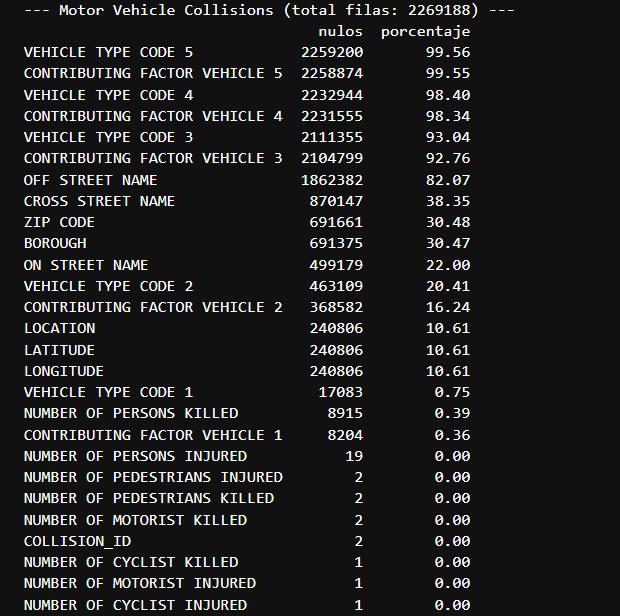
\includegraphics[width=\linewidth]{imagenes/image2.png}
    \end{minipage}
    \caption{Conteo y porcentaje de valores nulos en NYPD Arrest Data (izq. arriba), NYCgov Poverty Measure (izq. abajo) y Motor Vehicle Collisions (der.).}
    \label{fig:eda_elemento1_nulos}
\end{figure}

\subsection{Elemento 2 --- Estadísticos descriptivos generales}
\label{subsec:eda_elemento2}

Se calcularon estadísticos descriptivos distribuidos (conteo, media, desviación estándar, mínimo y máximo) mediante \texttt{.describe()} sobre variables numéricas clave de cada dataset. Para \textit{NYPD Arrest Data}, el precinto promedio de arresto es $63.41$ (desviación estándar de $34.01$, rango de $1$ a $123$), pero en las coordenadas planas estatales se detectó un mínimo anómalo de $-74$ en \texttt{X\_COORD\_CD} y de $40$ en \texttt{Y\_COORD\_CD}, valores que corresponden a latitud/longitud en grados decimales truncados y no a pies del sistema NAD 83. Para \textit{Motor Vehicle Collisions}, luego de aplicar conversión segura (\texttt{try\_cast}) sobre los conteos de víctimas, el promedio de personas heridas por colisión es $0.338$ ($\text{DE} = 0.722$, máximo $43$) y el de personas fallecidas es $0.00162$ ($\text{DE} = 0.0426$, máximo $8$).

\begin{figure}[H]
    \centering
    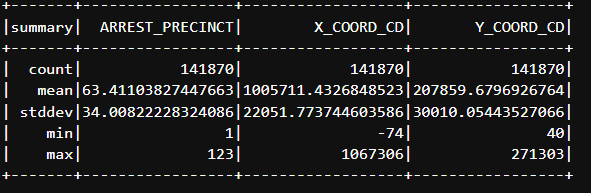
\includegraphics[width=0.75\textwidth]{imagenes/image4.png}\\[0.3cm]
    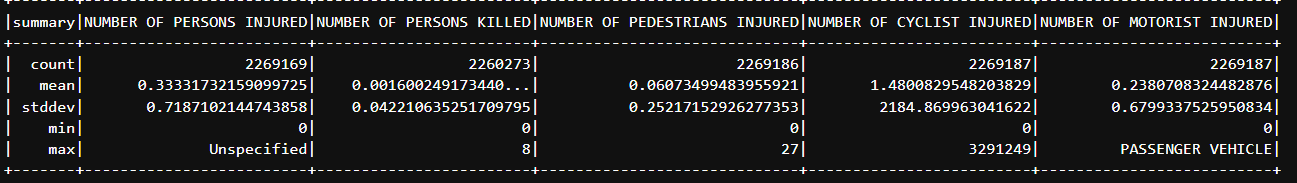
\includegraphics[width=0.95\textwidth]{imagenes/image5.png}
    \caption{Estadísticos descriptivos distribuidos (\texttt{.describe()}) para variables numéricas de arrestos y siniestros viales.}
    \label{fig:eda_elemento2_describe}
\end{figure}

\subsection{Elemento 3 --- Arrestos por Borough}
\label{subsec:eda_elemento3}

Brooklyn (\texttt{K}) concentra la mayor cantidad absoluta de arrestos con $42,877$ casos, seguido de Bronx (\texttt{B}) con $32,682$, Manhattan (\texttt{M}) con $32,089$, Queens (\texttt{Q}) con $29,053$ y, muy por debajo, Staten Island (\texttt{S}) con $5,169$. Esta distribución absoluta responde tanto al tamaño demográfico de cada condado como a la intensidad de patrullaje policial, motivo por el cual en la Sección \ref{sec:limpieza_transformacion} se estandariza por cada $100,000$ habitantes.

\begin{figure}[H]
    \centering
    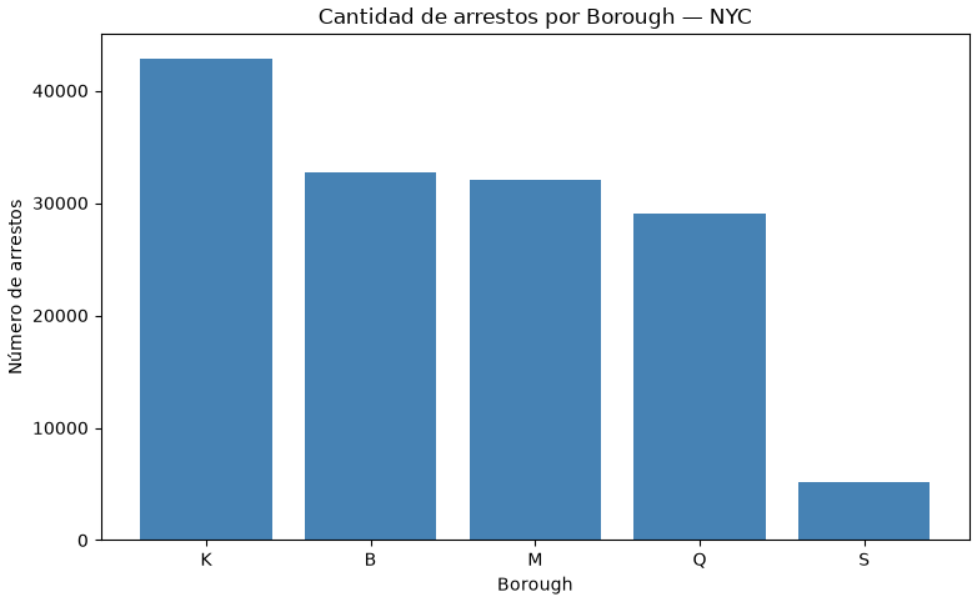
\includegraphics[width=0.75\textwidth]{imagenes/image6.png}
    \caption{Distribución absoluta de arrestos por condado (\textit{Borough}).}
    \label{fig:eda_elemento3_borough}
\end{figure}

\subsection{Elemento 4 --- Distribución de arrestos por nivel de gravedad de la ofensa}
\label{subsec:eda_elemento4}

El $58.5\%$ de los arrestos corresponden a delitos menores (\textit{misdemeanor}, \texttt{M}: $82,929$ casos), el $39.2\%$ a delitos graves (\textit{felony}, \texttt{F}: $55,651$ casos) y el $1.3\%$ a contravenciones (\textit{violation}, \texttt{V}: $1,896$ casos). Adicionalmente, se identificaron $864$ registros sin clasificación (\texttt{NaN}), $426$ registros con el código atípico \texttt{'9'}, $99$ con el código \texttt{'I'} (infracciones de tránsito/administrativas fuera de la tríada penal \texttt{F/M/V}) y $5$ con el texto \texttt{'(null)'}, sumando $1,394$ registros que se tratan en la fase de limpieza.

\begin{figure}[H]
    \centering
    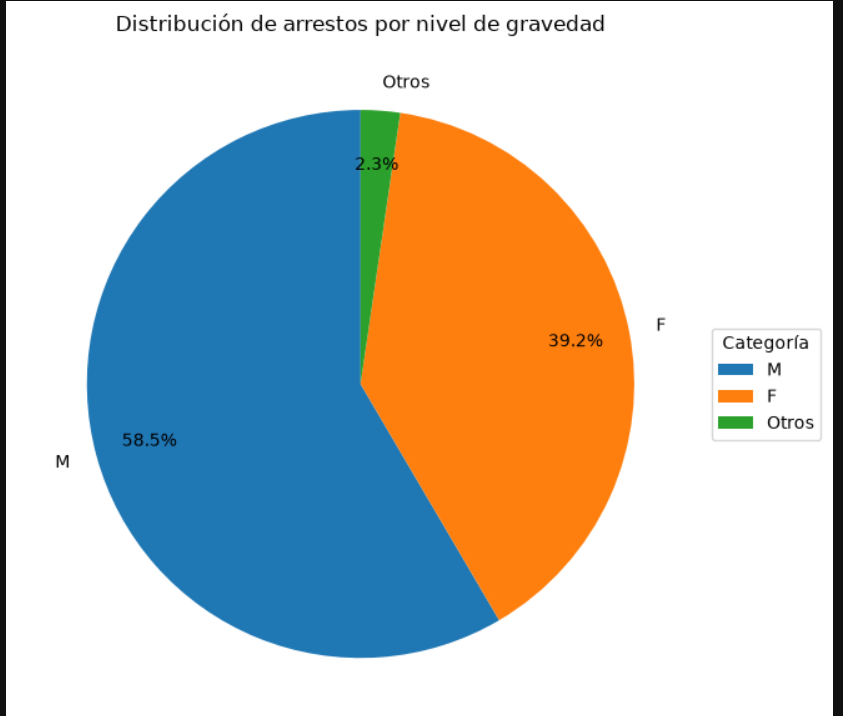
\includegraphics[width=0.75\textwidth]{imagenes/image7.png}
    \caption{Distribución de arrestos por nivel de gravedad de la ofensa (\texttt{LAW\_CAT\_CD}).}
    \label{fig:eda_elemento4_gravedad}
\end{figure}

\subsection{Elemento 5 --- Serie temporal de arrestos por mes}
\label{subsec:eda_elemento5}

Los arrestos mensuales muestran un comportamiento estable durante el primer semestre de 2026: enero registró $23,542$ detenciones, febrero presentó el punto más bajo ($21,069$, asociado también al menor número de días del mes), marzo subió a $24,696$, abril y mayo alcanzaron el máximo semestral prácticamente empatados ($25,129$ y $25,128$ respectivamente) y junio cerró en $22,306$ registros.

\begin{figure}[H]
    \centering
    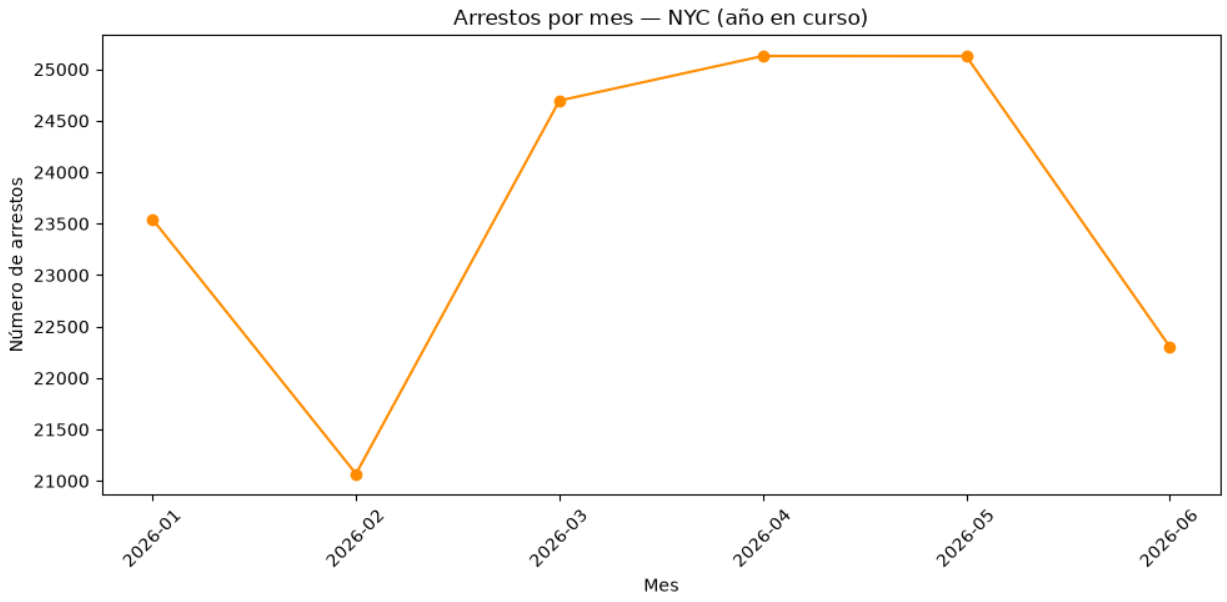
\includegraphics[width=0.70\textwidth]{imagenes/image8.png}
    \caption{Serie temporal mensual de arrestos en la Ciudad de Nueva York (enero a junio de 2026).}
    \label{fig:eda_elemento5_serie_temporal}
\end{figure}

\subsection{Elemento 6 --- Distribución de arrestos por grupo etario}
\label{subsec:eda_elemento6}

El grupo etario de \texttt{25-44} años concentra la mayoría de los arrestos con $81,521$ registros (equivalente al $57.46\%$ del total), seguido por el grupo de \texttt{45-64} años ($30,611$ registros, $21.58\%$) y el de \texttt{18-24} años ($20,946$ registros, $14.76\%$). Los extremos etarios (\texttt{<18} y \texttt{65+}) representan una proporción mucho menor ($5,587$ y $3,205$ arrestos, respectivamente).

\begin{figure}[H]
    \centering
    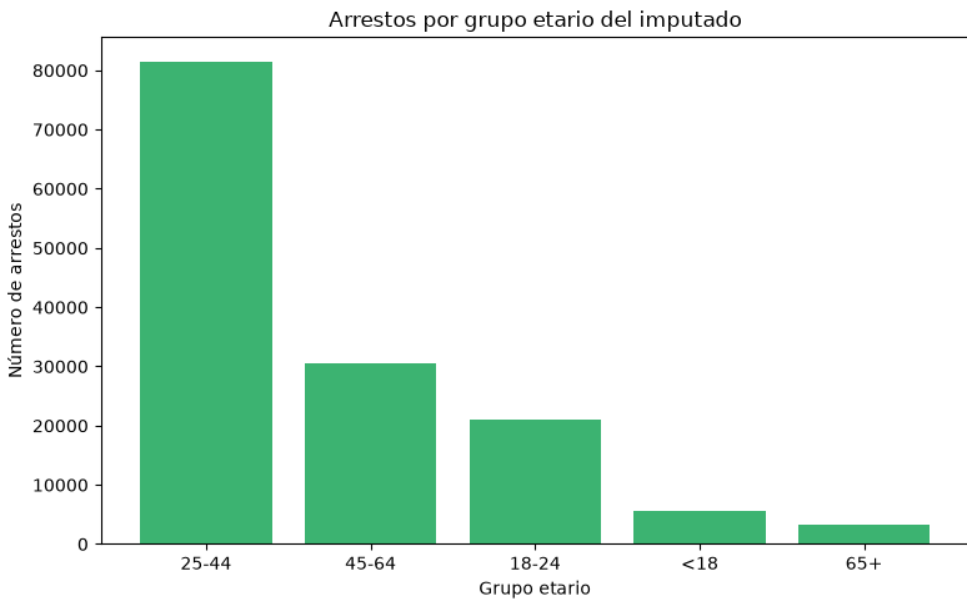
\includegraphics[width=0.65\textwidth]{imagenes/image9.png}
    \caption{Distribución de arrestos por grupo etario del imputado (\texttt{AGE\_GROUP}).}
    \label{fig:eda_elemento6_edad}
\end{figure}

\subsection{Elemento 7 --- Top 10 precincts con más arrestos}
\label{subsec:eda_elemento7}

El precinto $75$ (\textit{East New York}, Brooklyn) lidera el volumen de detenciones de toda la ciudad con $5,341$ arrestos, seguido del precinto $14$ (\textit{Midtown South}, Manhattan) con $4,382$ y el precinto $40$ (\textit{Mott Haven}, Bronx) con $4,061$. Completan los diez primeros lugares los precintos $46$ ($3,951$), $44$ ($3,882$), $103$ ($3,837$), $73$ ($3,524$), $52$ ($3,409$), $47$ ($3,084$) y $110$ ($3,001$), concentrados principalmente en el sur y centro del Bronx, el este de Brooklyn y el centro comercial de Manhattan.

\begin{figure}[H]
    \centering
    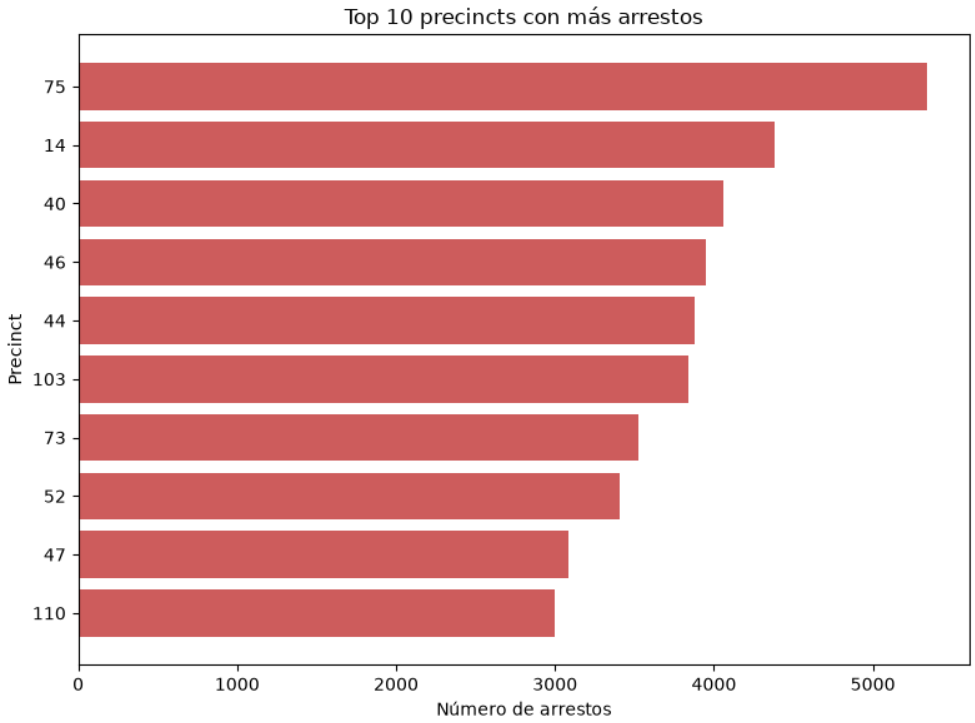
\includegraphics[width=0.75\textwidth]{imagenes/imagea.png}
    \caption{Top 10 distritos policiales (\textit{precincts}) con mayor volumen de arrestos.}
    \label{fig:eda_elemento7_top_precincts}
\end{figure}

\subsection{Elemento 8 --- Severidad de colisiones por tipo de persona involucrada (detección de registros desplazados)}
\label{subsec:eda_elemento8}

En la lectura exploratoria sin filtro de coherencia ni opción multilínea (Figura \ref{fig:eda_elemento8_severidad}), se detectó una anomalía crítica de calidad de datos: la suma de heridos por categoría superaba varias veces el total general de personas heridas debido a filas desplazadas por saltos de línea o comillas dentro de las direcciones, donde el identificador de colisión (\texttt{COLLISION\_ID} $\approx 3,291,249$) caía por error en la columna \texttt{NUMBER OF CYCLIST INJURED}. Este hallazgo motivó directamente la regla de lectura multilínea y el filtro de coherencia aritmética implementados en la Sección \ref{sec:limpieza_transformacion} (donde se presenta la distribución depurada real con $779,372$ heridos y $3,746$ fallecidos en la Figura \ref{fig:severidad_colisiones_limpia}).

\begin{figure}[H]
    \centering
    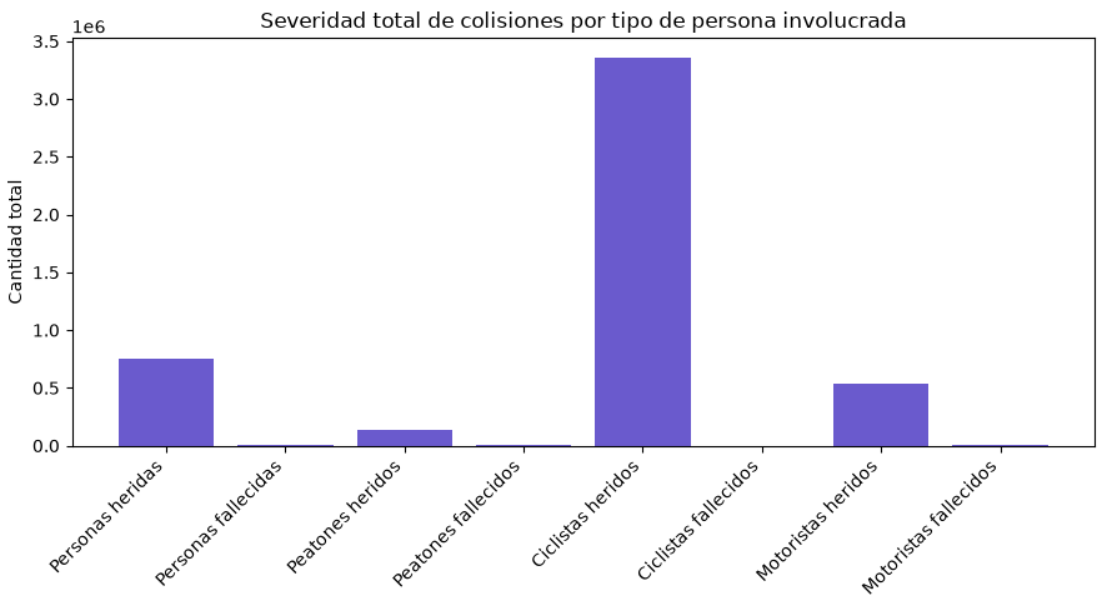
\includegraphics[width=0.85\textwidth]{imagenes/imageb.png}
    \caption{Inconsistencia detectada en la lectura preliminar de severidad de colisiones antes de aplicar el filtro de coherencia aritmética.}
    \label{fig:eda_elemento8_severidad}
\end{figure}

\subsection{Elemento 9 --- Cruce exploratorio entre tasa de pobreza y arrestos por Borough}
\label{subsec:eda_elemento9}

Al homologar los códigos de condado entre la encuesta de pobreza y los arrestos (Figura \ref{fig:eda_elemento9_pobreza_arrestos}), el Bronx presenta la mayor proporción muestral de pobreza ($25.79\%$), seguido de Brooklyn ($18.26\%$), Queens ($15.84\%$), y Manhattan y Staten Island ($13.83\%$ cada uno). En conteos brutos sin ponderar por población, Brooklyn registra más arrestos ($42,877$) que el Bronx ($32,682$); esta distorsión por tamaño poblacional se corrige en la Sección \ref{sec:limpieza_transformacion} mediante los factores de expansión \texttt{PWGTP}.

\begin{figure}[H]
    \centering
    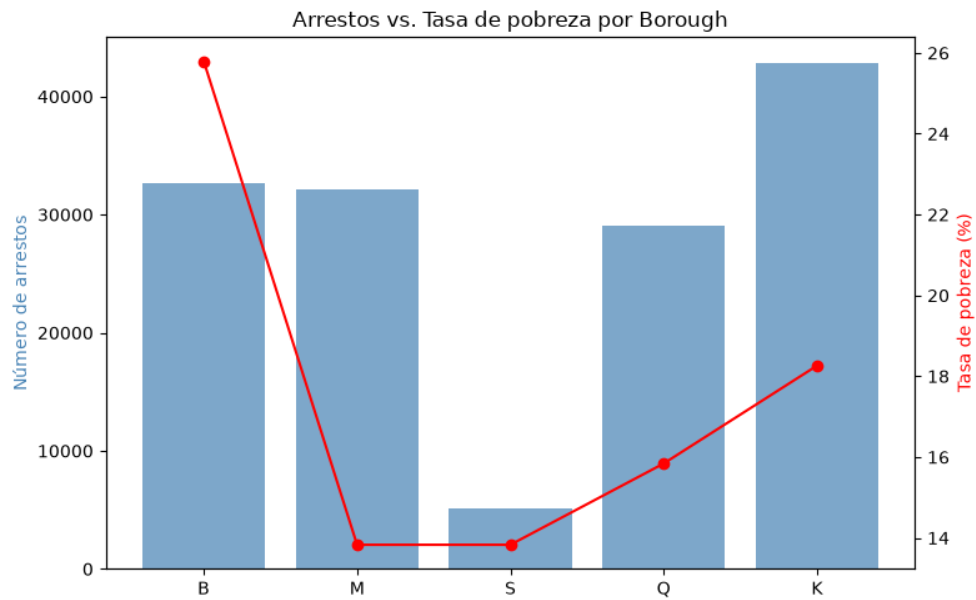
\includegraphics[width=0.8\textwidth]{imagenes/imagec.png}
    \caption{Cruce exploratorio inicial entre proporción muestral de pobreza y volumen bruto de arrestos por Borough.}
    \label{fig:eda_elemento9_pobreza_arrestos}
\end{figure}
